\documentclass[11pt,a4paper]{article}
\usepackage[margin=1.65cm]{geometry}
\usepackage{amsmath,amssymb,booktabs,array,xcolor,tikz,enumitem,microtype,hyperref,fancyhdr,titlesec}
\definecolor{navy}{HTML}{183153}\definecolor{blue}{HTML}{2E6F9E}\definecolor{pale}{HTML}{EEF4F8}\definecolor{warn}{HTML}{FFF3D6}
\hypersetup{colorlinks=true,linkcolor=blue,urlcolor=blue}
\pagestyle{fancy}\fancyhf{}\lhead{GCSE Physics · Current \& Voltage}\rhead{19 July 2026}\cfoot{\thepage}
\titleformat{\section}{\Large\bfseries\color{navy}}{}{0pt}{}[\color{blue}\titlerule]
\titleformat{\subsection}{\large\bfseries\color{blue}}{}{0pt}{}
\setlist{nosep,leftmargin=*}\setlength{\parindent}{0pt}\setlength{\parskip}{5pt}
\newcommand{\key}[1]{\colorbox{pale}{\parbox{0.96\linewidth}{#1}}}
\newcommand{\trap}[1]{\colorbox{warn}{\parbox{0.96\linewidth}{#1}}}
\begin{document}
\begin{center}
{\Huge\bfseries\color{navy} GCSE Physics — Electric Current \& Voltage in Resistors}\par\vspace{5pt}
{\large Student: Phuc Nguyen \quad Tutor: Alex Kealy \quad Date: 2026-07-19}\par\vspace{4pt}
\textit{Source: Loom recording (full video analysis) + transcript}
\end{center}
\key{\textbf{Evidence boundary.} This was a short, approximately nine-minute revision session. The guide therefore concentrates on the two fully recorded series-circuit questions and two spoken Ohm's-law checks. The later numerical answers are transparent completions of the recorded givens; the transcript does not preserve a spoken student result. Parallel-circuit rules were explicitly deferred and are not taught here.}

\section{The lesson's central idea: separate charge flow from energy transfer}
Two quantities were deliberately kept distinct. \textbf{Current}, $I$, describes the rate at which electric charge passes a point. \textbf{Potential difference}, $V$, describes energy transferred per unit charge between two points or across a component. This distinction explains why current can remain the same around a simple series loop while the potential difference is shared between resistors.

Phuc described current as ``charges per second'' and reasoned that the charge carriers continue around the loop even though their energy changes. Alex confirmed this. In GCSE notation the definition is
\[
\boxed{I=\frac{Q}{t}},
\]
where $I$ is in amperes (A), charge $Q$ is in coulombs (C), and time $t$ is in seconds (s). One ampere means one coulomb of charge passes a point each second. The formula supports the lesson reasoning; it was not used for a numerical calculation in this short recording.

\section{Current in a simple series circuit}
A series circuit has one unbranched path. Charge cannot disappear into a component or accumulate steadily at one position. In a steady circuit, the rate of charge flow into each resistor must therefore equal the rate leaving it. Hence
\[
\boxed{I_{\text{before}}=I_{\text{between}}=I_{\text{after}}}.
\]

\begin{center}
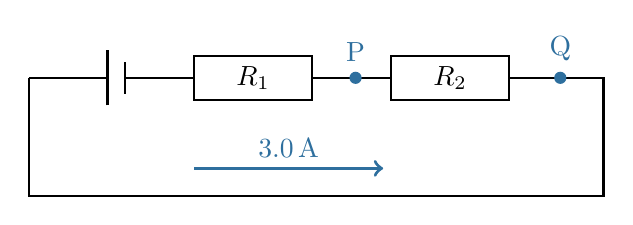
\begin{tikzpicture}[x=1cm,y=1cm,thick]
\draw (0,0)--(1,0);\draw (1,-.35)--(1,.35);\draw (1.22,-.2)--(1.22,.2);\draw (1.22,0)--(2.1,0);
\draw (2.1,-.28) rectangle (3.6,.28);\node at (2.85,0){$R_1$};
\draw (3.6,0)--(4.6,0);\fill[blue] (4.15,0) circle (2.2pt);\node[above,blue] at (4.15,.08){P};
\draw (4.6,-.28) rectangle (6.1,.28);\node at (5.35,0){$R_2$};
\draw (6.1,0)--(7.3,0)--(7.3,-1.5)--(0,-1.5)--(0,0);
\fill[blue] (6.75,0) circle (2.2pt);\node[above,blue] at (6.75,.08){Q};
\draw[->,blue,very thick] (2.1,-1.15)--(4.5,-1.15) node[midway,above]{$3.0\,\mathrm{A}$};
\end{tikzpicture}
\end{center}

\subsection{Recorded question 1 (00:43--01:57)}
The displayed loop contained a battery and two resistors in series. The diagram gave a current of $3.0\,\mathrm{A}$ and asked for the current at P, between the resistors, and Q, after the second resistor.

Phuc answered P as 3 A, correctly naming amperes, then said Q should also be the same because ``the current is supposed to be the same everywhere.'' Alex confirmed both answers and the charge-flow explanation. Therefore
\[
\boxed{I_P=3.0\,\mathrm{A}},\qquad \boxed{I_Q=3.0\,\mathrm{A}}.
\]
\textbf{Sense check:} if the second resistor somehow received less charge per second than the first, charge would pile up between them. That is not the steady series circuit shown.

\trap{\textbf{Common mistake.} Do not say that a resistor ``uses up current.'' A resistor transfers energy from the electrical store, but charge still flows through it. In this simple series loop the current is the same on both sides.}

\section{Potential difference across series resistors}
The source supplies energy per coulomb; the resistors transfer that energy. For the two-resistor series circuit in the lesson, energy conservation gives
\[
\boxed{V_{\text{source}}=V_1+V_2}.
\]
This is why the individual potential differences may differ while their sum cannot exceed the source value in the closed loop being considered.

\begin{center}
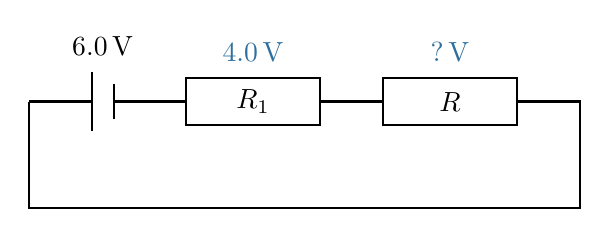
\begin{tikzpicture}[x=1cm,y=1cm,thick]
\draw (0,0)--(.8,0);\draw (.8,-.38)--(.8,.38);\draw (1.08,-.22)--(1.08,.22);\node[above] at (.94,.45){$6.0\,\mathrm{V}$};\draw (1.08,0)--(2,0);
\draw (2,-.3) rectangle (3.7,.3);\node at (2.85,0){$R_1$};\node[above,blue] at (2.85,.38){$4.0\,\mathrm{V}$};
\draw (3.7,0)--(4.5,0);\draw (4.5,-.3) rectangle (6.2,.3);\node at (5.35,0){$R$};\node[above,blue] at (5.35,.38){$?\,\mathrm{V}$};
\draw (6.2,0)--(7,0)--(7,-1.35)--(0,-1.35)--(0,0);
\end{tikzpicture}
\end{center}

\subsection{Recorded question 2 (03:15--05:26)}
The source was $6.0\,\mathrm{V}$. One resistor had $4.0\,\mathrm{V}$ across it; the question asked for the potential difference across resistor $R$. Phuc first replied ``4,'' reading back the known label rather than the requested unknown. Alex refocused the question: six volts are supplied, four volts are across the first resistor, so how many are left across $R$?
\begin{align*}
V_{\text{source}}&=V_1+V_R,\\
6.0&=4.0+V_R,\\
V_R&=6.0-4.0=\boxed{2.0\,\mathrm{V}}.
\end{align*}
Alex described an electron leaving the source with six volts' worth of energy per charge, transferring four across the first resistor and two across the second. More precisely, voltage is energy transferred \emph{per coulomb}; the story is a useful bookkeeping picture, not a claim that a single electron races around carrying all the energy itself. Alex immediately added that individual electrons drift slowly and compared the circuit with pulling a rope: energy transfer through the established circuit is not the same as one electron travelling quickly all the way around.

\trap{\textbf{Common mistake.} Read the component label the question names. The visible $4.0\,\mathrm{V}$ belonged to the first resistor; it was a given used to find the unknown across $R$, not the answer. Also use volts (V), not ``voltage,'' as the unit.}

\section{Connecting voltage, current and resistance}
The final minutes used the resistance relationship
\[
\boxed{V=IR},\qquad R=\frac{V}{I},\qquad I=\frac{V}{R}.
\]
Voltage is measured in volts (V), current in amperes (A), and resistance in ohms ($\Omega$). Before substituting, identify the required quantity and rearrange the equation. This avoids dividing the wrong way.

\subsection{Spoken check A: total resistance}
Using the same $6.0\,\mathrm{V}$ source, Alex gave a total current of $3.7\,\mathrm{A}$ and asked for the total resistance. The transcript records Phuc recalling the unit, ohms, but not a spoken numerical answer. Completing the recorded givens:
\[
R_{\text{total}}=\frac{V}{I}=\frac{6.0}{3.7}=1.6216\ldots\,\Omega\approx\boxed{1.6\,\Omega}\quad(2\text{ s.f.}).
\]
\textbf{Check:} $IR\approx(3.7)(1.6)=5.92\,\mathrm{V}$, which rounds consistently to $6.0\,\mathrm{V}$.

\subsection{Spoken check B: current}
Alex then stated a resistance of $6000\,\Omega$ and an emf of $25\,\mathrm{V}$, asking for current. Again, no spoken result survives in the transcript, so the calculation below is a labelled completion:
\[
I=\frac{V}{R}=\frac{25}{6000}=0.004166\ldots\,\mathrm{A}\approx\boxed{4.2\times10^{-3}\,\mathrm{A}}=\boxed{4.2\,\mathrm{mA}}.
\]
\textbf{Scale check:} a resistance of thousands of ohms with only tens of volts should give a small current, so a few milliamperes is sensible.

\section{Fast method and mistake-proof checks}
\begin{enumerate}
\item Decide whether the question is about \textbf{charge flow} (current), \textbf{energy per charge} (potential difference), or the link $V=IR$.
\item For an unbranched series loop, copy the same current to every position.
\item For series voltage, write the source as the sum across components, then subtract the known share.
\item For resistance calculations, write $V=IR$, rearrange symbolically, substitute, and include the unit.
\item Check the result: series voltages add to the source; substituting $I$ and $R$ should recover $V$; a large resistance should suppress current for fixed voltage.
\end{enumerate}

\section{Quick recall}
\begin{tabular}{p{5.2cm}p{9.2cm}}
\toprule Prompt & Retrieval answer \\ \midrule
What is current? & Rate of flow of charge: $I=Q/t$, measured in A. \\
Current at different points in one series loop? & The same everywhere in the steady unbranched loop. \\
What does potential difference track? & Energy transferred per unit charge, measured in V. \\
How are series potential differences linked? & They add to the source: $V_{\text{source}}=\sum V_{\text{components}}$. \\
Resistance relationship? & $V=IR$; rearrange for the requested quantity. \\
What was deferred? & Parallel-circuit rules; Alex said they could revise circuit rules next time. \\ \bottomrule
\end{tabular}

\section{Question coverage ledger}
\begin{tabular}{p{5cm}p{2.3cm}p{7.1cm}}
\toprule Discussion & Status & Preserved outcome \\ \midrule
Current at P and Q in a $3.0$ A series circuit & Solved & Phuc answered both correctly and explained charge conservation; Alex confirmed. \\
Unknown voltage in a $6.0$ V, $4.0$ V series circuit & Solved after correction & Phuc first read the known 4 V; Alex redirected; Phuc reached 2 V. \\
Total $R$ for $6.0$ V and $3.7$ A & Discussed; completion labelled & Givens and requested unit survive; $R\approx1.6\,\Omega$ is calculated transparently here. \\
Current for $25$ V and $6000\,\Omega$ & Discussed; completion labelled & Givens survive; $I\approx4.2\,\mathrm{mA}$ is calculated transparently here. \\
Parallel circuits & Deferred & Tutor said this had not yet been revised; no parallel rule is invented. \\ \bottomrule
\end{tabular}
\end{document}
